\documentclass[12pt,letterpaper, onecolumn]{exam}
\usepackage{amsmath}
\usepackage{amssymb}
\usepackage{graphicx}
\usepackage{float}
\usepackage{longtable}
\usepackage{booktabs}
\usepackage[utf8]{inputenc}
\usepackage[russian]{babel}
\usepackage[lmargin=60pt, rmargin=60pt, tmargin=1.2in]{geometry}  %For centering solution box
\usepackage{xcolor}
% \chead{\hline} % Un-comment to draw line below header
\thispagestyle{empty}   %For removing header/footer from page 1
\usepackage{listings}
\usepackage{xcolor}

\lstdefinestyle{sparkconf}{
  basicstyle=\ttfamily\small,
  backgroundcolor=\color{gray!10},
  frame=single,
  breaklines=true,
  captionpos=b
}

\lstdefinestyle{pythoncode}{
  language=Python,
  basicstyle=\ttfamily\footnotesize,
  backgroundcolor=\color{gray!10},
  frame=single,
  breaklines=true,
  keywordstyle=\color{blue!70!black},
  stringstyle=\color{green!50!black},
  commentstyle=\color{gray!60!black}\itshape,
  showstringspaces=false,
  captionpos=b
}

\begin{document}

\begingroup  
    \centering
    \LARGE Экспериментальная актуализация научной статьи "Research and experimental analysis of Big Data tools: an application for Twitch streaming platform" \\[0.5em]
    \large  2026\\[0.5em]
    \large Фролов Георгий Оскарович\par
    \large ITMO | AI Talent Hub\par
\endgroup
\rule{\textwidth}{0.7pt}
\pointsdroppedatright   %Self-explanatory
\printanswers
\renewcommand{\solutiontitle}{\noindent\textbf{Ans:}\enspace}   %Replace "Ans:" with starting keyword in solution box

\section{Введение}

В 2024 году я заканчивал обучение на бакалавриате в СПбПУ по специальности "Прикладная информатика". Тема моего диплома была следующая: "Исследование и экспериментальный анализ средств работы с большими данными в веб-приложениях". Суть работы по сути заключалась в сборе текстовых сообщений из чатов Twitch(нужен был какой-то релевантный источник данных для работы) агрегации их в HDFS и выполнении на них расчетов двух типов: пакетного и потокового. В рамках потоковой обработки данных, которая выполнялась сразу при получении данных из IRC сокета и перенаправления его в Kafka топик, сравнивались Spark Streaming и Apache Flink. К текущей работе это не имеет отношение, помимо того, что после того, как сообщение обрабатывалось потоковым фреймворком - оно сохранялось в HDFS и становилось частью источника для пакетной обработки данных.

В пакетной же обработке данных сравнивались Hive On Tez, Spark и Hadoop MapReduce. Все расчеты проводились на моем ноутбуке в local/pseudo-cluster режимах. Ну и главный минус - объемы данных были такими, что назвать их "большими данными" язык бы не повернулся - 346, 683 и 2350 Мб для датасетов Small, Medium и Large соответственно. Позже, мы с моим научным руководителем решили написать статью по моему диплому, и с этой статьей осенью 2025 года я выступал на конференции по большим данным, справедливо столкнувшись в конце выступления с вопросом про объем данных - действительно ли я считаю, что они "большие"?

Тогда я вынужден был признать, что "большими" они не являются, вместе с тем решив, что просто так это оставлять нельзя, и стоит повторить эксперимент на данных, которые можно назвать "большими" хотя бы без иронии. Собственно \textbf{в данной работе мы будем} повторять эксперименты пакетной обработки данных, т.е. выполнять обозначенные запросы на датасетах разного размера и сравнивать время выполнения, отмечу только, что Hadoop MapReduce мы из сравнения исключим, так как еще в той работе было выявлено, что он необратимо устарел и показывает очень слабую производительность по сравнению с Hive On Tez и Spark.

Также благодаря этому диплому и наличию в дипломной комиссии сотрудника одного из крупных банков, я получил работу Дата-инженером в этом банке, собственно благодаря этому у меня и есть возможность провести эксперименты по новой, на б\'oльших объемах данных, так что все очень удобно. Кроме того, с этим сравнением(Hive On Tez vs Spark) я сталкиваюсь каждый день в ходе выполнения рабочих задач, так как у меня есть набор корпоративных инструментов для выполнения моих обязанностей, один из них работает с данными через Hive On Tez, второй через Spark, и я по сути каждый день делаю выбор между ними в зависимости от задачи)

В ближайшем будущем по на основе этого отчета можно будет написать новую статью, выступающую как актуализацию/более релевантную версию предыдущей статьи(с исключением экспериментов по потоковой обработки). Но это уже конечно зависит от результатов практики...

Далее опишем методологию проведения экспериментов, она будет разбита на несколько сегментов, которые я считаю важными описать достаточно подробно, чтобы результаты экспериментов можно было считать релевантными. Приступим.

\section{Методология}

Как я уже сказал, описание методологии нужно разбить на несколько секций, но все они служат одной цели - подтвердить легитимность, адекватность, воспроизводимость, в целом - состоятельность проводимого сравнения.

Обозначу, что метрикой для экспериментов будет время выполнения запроса. Далее подробнее обозначим, что именно под этим имеется в виду.

\subsection{Данные}

Начнем с описания новых данных. Главное для данной работы - чтобы данные были "большими", в противном случае работа не будет иметь смысла. Также неплохо, чтобы данные были "реальными" - не синтетическими. Так как я выполняю расчеты на рабочих средах, и моя предметная область на работе - контракты, мной был выбран источник данных zakupki.gov.ru. Это сайт с данными о государственных контрактах и любой контракт, который государственное учреждение заключает должен быть отражен в реестре zakupki.gov.ru согласно 44 ФЗ/223 ФЗ. Сами данные по контрактам поставляются в мою организацию третьим специализированным источником, но я взаимодействую с ними как с партицированными хранящимися в HDFS в формате parquet данными.
На данный момент в моем распоряжении данные о 25.5 миллионах контрактов, при этом данные разбиты на несколько сущностей, контракты - родительская сущность, а самая многочисленная из них - документы по контракту. На данный момент на 25.5 миллионов контрактов приходится 414.4 миллионов документов, т.е. в среднем \~16 документов на контракт. Плюс "реальности" данных в данном случае означает наличие "перекосов", которыми обладают реальные данные, в следствие чего сравнение будет более репрезентативным.

Сами по себе таблицы, несмотря на большое количество записей, весят недостаточно для достижения заявленных в мотивации к работе показателей объема данных. Но контракты и документы это просто разные сущности, хранящиеся в нормализованном виде, чтобы достичь необходимых объемов таблиц, мы можем их сджойнить, причем не как-то "рандомно", а семантически верно, по ключу - реестровому номеру контракта (каждый документ относится к контракту с конкретным номером, который является уникальным идентификатором контракта). После такого джойна мы получаем достаточно данных, и даже больше чем нужно, на практике пришлось отбирать сэмплы нужного размера. 

Формат хранения данных я определял сам, так как мне необходимо было копировать данные в мою схему для того, чтобы иметь контроль над hive metastore для сбора статистики по таблицам, выбрал следующий сетап - parquet по 200 партиций на каждый из датасетов. Фиксированное число партиций в нашем случае - наиболее адекватный подход, это превышает максимальной число executorов и в Spark и в Hive On Tez, а также позволит избежать неверной трактовки времени выполнения за счет увеличения числа партиций с ростом объема данных (такой же подход будет применяться и при выставлении ресурсов при проведении экспериментов, об этом - в следующем сегменте).

По итогу работ по подготовке данных для проведения экспериментов была получена таблица со следующей схемой:

\begin{longtable}{|p{4.5cm}|p{2cm}|p{8cm}|p{2cm}|}
\caption{Схема таблиц — источников данных для экспериментов}
\label{tab:schema} \\
\hline
\textbf{Атрибут} & \textbf{Тип данных} & \textbf{Описание} & \textbf{Исходная сущность} \\
\hline
\endfirsthead
\hline
\textbf{Атрибут} & \textbf{Тип данных} & \textbf{Описание} & \textbf{Исходная сущность} \\
\hline
\endhead
\hline
\endfoot
contract\_reg\_num & string & Реестровый номер контракта & Контракт \\
stage\_start\_contract & string & Этап контракта (дата начала) & Документ \\
stage\_end\_contract & string & Этап контракта (дата окончания) & Документ \\
docs\_done\_stage & string & Документы, подтверждающие исполнение контракта & Документ \\
doc\_type & string & Тип документа, подтверждающего исполнение контракта & Документ \\
doc\_url & string & Ссылка на документ, подтверждающий исполнение контракта & Документ \\
dt\_signing & string & Дата подписания документа & Документ \\
cost\_done & string & Стоимость исполненных поставщиком обязательств & Документ \\
paid\_act\_stage & string & Фактически оплачено & Документ \\
inf\_nonexecution\_contract & string & Информация о ненадлежащем исполнении или неисполнении контракта & Контракт \\
object\_tender & string & Объект закупки & Контракт \\
delivered\_goods & string & Количество поставленных товаров, выполненных работ, оказанных услуг & Контракт \\
object\_cost & string & Стоимость исполненных обязательств & Контракт \\
supplier\_inn & string & ИНН поставщика & Контракт \\
supplier\_name & string & Наименование поставщика & Контракт \\
price & string & Цена контракта & Контракт \\
currency & string & Валюта контракта & Контракт \\
dt\_contract & string & Дата заключения контракта & Контракт \\
start\_dt\_contract & string & Дата начала выполнения работ по контракту & Контракт \\
end\_dt\_contract & string & Дата завершения выполнения работ по контракту & Контракт \\
customer\_inn & string & ИНН заказчика & Контракт \\
status & string & Статус исполнения контракта & Контракт \\
termination\_cause & string & Основание расторжения контракта & Контракт \\
termination\_dt & string & Дата расторжения контракта & Контракт \\
reason\_termination & string & Причина расторжения контракта & Контракт \\
type & string & Тип контракта & Контракт \\
customer\_name & string & Наименование заказчика & Контракт \\
reason\_change & string & Причина изменения условий контракта & Контракт \\
doc\_change & string & Реквизиты документа, являющегося основанием изменения условия контракта & Контракт \\
doc\_termination & string & Документ, являющийся основанием расторжения контракта & Контракт \\
termination\_dt\_court & string & Дата расторжения контракта по суду & Контракт \\
contract\_num & string & Номер контракта & Контракт \\
contract\_subject & string & Предмет контракта & Контракт \\
notification\_number & string & Реестровый номер закупки & Контракт \\
bank\_support & string & Информация о банковском и (или) казначейском сопровождении контракта & Контракт \\
advance\_percent & string & Размер аванса в процентах & Контракт \\
advance\_rub & string & Размер аванса в рублевом эквиваленте & Контракт \\
contract\_subject\_2 & string & Предмет контракта & Контракт \\
supplier\_account & string & Номер банковского казначейского счета & Контракт \\
\hline
\end{longtable}

Как можно заметить, все типы данных string, что свидетельсвует о том, что это "сырые" данные. Это тоже неплохая характеристика, на них можно проделать много "типичных" дата-инженерных задач, что часто происходило у меня во время работы.

В некоторых экспериментах будут использоваться и другие таблицы помимо этих, просто для того, чтобы было, с чем joinить, важные для конкретного эксперимента характеристики таблиц будут описаны "рядом" с экспериментом.

Структуру данных мы разъяснили, перейдём к объему. Было создано три датасета со следующими характеристиками:

\begin{table}[ht]
\centering
\caption{Описание сформированных наборов данных}
\label{tab:datasets}
\begin{tabular}{lrr}
\toprule
\textbf{Имя таблицы} & \textbf{Количество записей} & \textbf{Объём (МБ)} \\
\midrule
contracts\_docs\_tiny  & 4046690  & 6758.4  \\
contracts\_docs\_medium & 99922159  & 172236.8  \\
contracts\_docs\_large  & 148617482 & 262656.0  \\
\bottomrule
\end{tabular}
\end{table}

Данные можно легитимно назвать "большими", учитывая ресурсы сред выполнения, которая будет описана в следующей главе. Проведение работы в контексте данных считаю оправданным.

\subsection{Среда выполнения и ресурсы}

Но только подходящих данных для успешной актуализации эксперимента недостаточно. Нужно еще погрузить сравниваемые инструменты в равные условия. В контексте Hive On Tez и Spark это означает уровнять их по ресурсам. Так как я провожу эксперименты на корпоративном оборудовании, по сути это означает, что я должен уровнять Hive On Tez и Spark по выделяемым ресурсам.

Прежде чем описывать настройку ресурсов, зафиксируем версии сравниваемых
инструментов, так как поведение оптимизаторов и адаптивных механизмов между
версиями существенно различается. Hive-on-Tez представлен версией 3.1.2
(вендорская сборка) поверх Apache Tez 0.10.2; в этой версии стоимостный
оптимизатор на основе Calcite (CBO) включён по умолчанию. Apache Spark
используется версии 3.5.1 - в ней адаптивная оптимизация (AQE) является зрелой и доступна из коробки, однако стоимостный оптимизатор (CBO) по умолчанию отключён и активируется явно.

Также стоит оговориться, что Hive On Tez получает ресурсы через YARN RM и берет ресурсы из коммунальной YARN очереди, в то время как Spark хостится на k8s кластере и его ресурсы ограничены квотой. Data-locality сопоставима на уровне стойки, так как по факту spark executorы в процессе выполнения запроса находятся на тех же рейках, что и Tez mapperы и reducerы, хотя node-locality может различаться. 

Ресурсы для Hive On Tez и Spark я могу контролировать в рамках сессий. Hive On Tez без регулирования получал бы 10\% дефолтной YARN очереди, в абсолютных цифрах значительно больше ресурсов, чем Spark - 368 ядер и 4.4Tb оперативки. Tez бы точно не задействовал все выделяемые ресурсы, учитывая объемы данных описанные в предыдущем сегменте, они значительно меньше. При этом Spark я использую в коммунальном сервисе с льготой 288GB executor RAM и 24 CPU.

Поэтому, чтобы "уровнять" инструменты по ресурсам для spark мы выставим статически алоцированный максимум доступных по квоте ресурсов:


\noindent
\begin{minipage}{\linewidth}
\begin{lstlisting}[style=sparkconf, caption={Конфигурация ресурсов Spark}, label={lst:spark-conf}]
spark.dynamicAllocation.enabled = false
spark.executor.instances        = 12
spark.executor.cores            = 2
spark.executor.memory           = 20g
spark.executor.memoryOverhead   = 4g
spark.driver.memory             = 8g
spark.driver.cores              = 2
\end{lstlisting}
\end{minipage}

\begin{table}[ht]
\centering
\caption{Конфигурация ресурсов Hive-on-Tez}
\label{tab:hive-conf}
\begin{tabular}{|l|l|p{6cm}|}
\hline
\textbf{Параметр} & \textbf{Значение} & \textbf{Назначение} \\
\hline
hive.tez.container.size & 12288 & Память одного Tez-контейнера, МБ \\
hive.tez.java.opts & -Xmx9830m & Heap внутри контейнера ($\approx$80\% от container.size) \\
hive.exec.reducers.max & 24 & Верхняя граница числа reduce-контейнеров \\
hive.tez.auto.reducer.parallelism & false & Жёсткая фиксация числа редьюсеров по потолку \\
tez.grouping.min-size & $V/24$ & Мин. размер input-сплита (под целевое число мапперов) \\
tez.grouping.max-size & $2V/24$ & Макс. размер input-сплита \\
\hline
\end{tabular}

\vspace{0.5em}
{\footnotesize где $V$ - объём тира; для каждого набора данных размер группировки пересчитывается, чтобы удерживать $\approx 24$ контейнера.}
\end{table}

В отличие от Spark, где число и размер исполнителей задаются напрямую и фиксируются на всё приложение, Hive-on-Tez распределяет ресурсы эластично: число контейнеров определяется планировщиком в зависимости от объёма обрабатываемых данных и степени параллелизма каждой фазы DAG. Поэтому привести Hive к заданному ресурсному бюджету можно лишь косвенно - через ограничение параллелизма обеих фаз обработки.

Ресурсное потребление Tez складывается из двух фаз. Число контейнеров reduce-фазы ограничивается параметром hive.exec.reducers.max. При hive.tez.auto.reducer.parallelism=false это значение трактуется как жёсткий потолок, а не как ориентир для автоподбора. Число контейнеров map-фазы напрямую не задаётся, а определяется размером входных сплитов: Tez группирует исходные файлы в сплиты целевого размера (tez.grouping.min-size/max-size), и каждый сплит обрабатывается одним контейнером. Таким образом, число мапперов обратно пропорционально размеру группировки:
\[
N_{map} \approx V / S_{group},
\]
где $V$ - объём данных, $S_{group}$ - размер сплита.

Это разделение существенно: при наблюдении за выполнением неограниченного запроса пиковое потребление приходилось именно на map-фазу - параллельное чтение порождало сотни одновременных контейнеров, тогда как ограничение reducers.max на эту фазу не влияет. Поэтому для удержания суммарного бюджета ограничиваются обе фазы независимо.

Размер контейнера фиксируется (hive.tez.container.size), а размер группировки подбирается под целевое число контейнеров $N$ для каждого набора данных:
\[
S_{group} = V / N.
\]
При фиксированном $N$ суммарный ресурсный бюджет ($N \times$ container.size) остаётся постоянным независимо от объёма данных. Это позволяет изолировать эффект роста объёма от эффекта изменения параллелизма - иначе рост числа контейнеров с объёмом исказил бы интерпретацию времени выполнения.

Целевой бюджет ($N = 24$ контейнера, $24 \times 12$~ГБ $\approx 288$~ГБ) выбран равным фиксированному бюджету Spark, что обеспечивает сопоставимость по совокупному объёму выделенных ресурсов. Фактическое потребление верифицировалось апостериори по агрегированным метрикам YARN (vcore-секунды, MB-секунды).

\subsection{Конфигурации сравнения и методика анализа}
\label{sec:configs}

Сравнение проводится в трёх конфигурациях, позволяющих разделить вклад движка
и вклад адаптивной оптимизации. Hive-on-Tez использует статическое
планирование на основе оптимизатора Calcite (CBO), при котором план строится
до выполнения по собранной статистике и далее не изменяется. Для Spark
рассматриваются два режима: с включённой адаптивной оптимизацией
(Adaptive Query Execution, AQE) и без неё. В обоих режимах в Spark
активирован стоимостный оптимизатор (CBO), опирающийся на ту же статистику.

Такое разбиение изолирует две независимые оси. Конфигурация Spark с выключенным
AQE концептуально симметрична Hive-on-Tez: оба движка строят план до выполнения
по статистике и не переписывают его в рантайме - сравнение этих режимов
характеризует различие движков как таковых. Конфигурация Spark с включённым AQE
добавляет переоптимизацию плана во время выполнения по фактическим данным
(в частности, обработку перекоса распределения ключей), что характеризует вклад
адаптивности. Соответствие конфигураций уровням оптимизации приведено
в табл.~\ref{tab:opt-matrix}.

\begin{table}[t]
\centering
\caption{Уровни оптимизации в сравниваемых конфигурациях}
\label{tab:opt-matrix}
\begin{tabular}{|l|l|l|}
\hline
\textbf{Конфигурация} & \textbf{План-тайм (CBO)} & \textbf{Рантайм (AQE)} \\
\hline
Spark, CBO-on / AQE-off & по статистике, фиксирован & нет адаптации \\
Spark, CBO-on / AQE-on  & по статистике & переписывается в рантайме \\
Hive-on-Tez             & Calcite по статистике & нет рантайм-адаптации \\
\hline
\end{tabular}
\end{table}

\subsubsection{Сбор статистики}
Стоимостный оптимизатор обоих движков опирается на статистику, собираемую
командой ANALYZE. Различаются два уровня: табличная статистика
(число строк и объём) и колоночная (кардинальность, экстремумы, доля
NULL), необходимая для оценки селективности соединений и группировок.
Статистика собиралась на рабочих наборах данных для ключевых атрибутов,
участвующих в соединениях, группировках и фильтрах.

\begin{lstlisting}[style=sparkconf, caption={Сбор статистики}, label={lst:analyze}]
ANALYZE TABLE t_team_amkld.contracts_docs_<tier> COMPUTE STATISTICS;
ANALYZE TABLE t_team_amkld.contracts_docs_<tier> COMPUTE STATISTICS
    FOR COLUMNS contract_reg_num, supplier_inn, customer_inn,
                dt_contract, price;
\end{lstlisting}

\subsubsection{Конфигурация Spark}
Стоимостный оптимизатор (CBO) активируется явно (по умолчанию в Spark он отключён);
адаптивная оптимизация переключается между двумя режимами.

\begin{lstlisting}[style=sparkconf, caption={Конфигурация CBO и AQE в Spark}, label={lst:spark-opt}]
# Cost based optimization
spark.sql.cbo.enabled                            = true
spark.sql.cbo.joinReorder.enabled                = true

# AQE-on
spark.sql.adaptive.enabled                       = true
spark.sql.adaptive.skewJoin.enabled              = true
spark.sql.adaptive.coalescePartitions.enabled    = true

# AQE-off
spark.sql.adaptive.enabled                       = false
\end{lstlisting}

\subsubsection{Процедура измерения}
Основной метрикой служит сквозное время выполнения (wall-clock), фиксируемое
от отправки запроса до получения результата. Для запросов, результат которых
не требуется сохранять, выполнение инициируется действием, вынуждающим полное
исполнение вычислительного плана без материализации результирующего набора
на диск: для запросов с агрегацией - подсчётом строк результата, для запросов
с полной проекцией (приведение типов) - записью в формат-приёмник noop,
не сохраняющий данные, но вынуждающий обработать все столбцы.

Для каждого запроса выполняется один <<холодный>> прогон и несколько
<<горячих>>. Холодный прогон соответствует первому обращению в рамках сессии
и включает накладные расходы на инициализацию исполнителей и компиляцию JIT;
он приводится отдельно. Итоговым значением служит медиана горячих прогонов,
устойчивая к единичным выбросам, характерным для разделяемого кластера, где
состояние страничного кэша и доступность ресурсов не контролируются.
Запросы Spark исполняются программно (листинг~\ref{lst:runner}); запросы Hive
выполняются через веб-интерфейс Hue, время фиксируется по журналу выполнения.

\begin{lstlisting}[style=pythoncode, caption={Обёртка запуска и измерения для Spark}, label={lst:runner}]
import time, csv, statistics

def run_query(spark, query, query_id, tier,
              n_hot=4, action="count", csv_writer=None):
    def execute():
        t0 = time.time()
        df = spark.sql(query)
        if action == "count":
            df.count()
        else:
            df.write.format("noop").mode("overwrite").save()
        return time.time() - t0

    cold = execute()
    hot_times = [execute() for _ in range(n_hot)]
    hot_median = statistics.median(hot_times)

    if csv_writer:
        csv_writer.writerow(["spark", query_id, tier,
                             round(hot_median, 3), round(cold, 3),
                             *[round(t, 3) for t in hot_times]])
    return hot_median, cold
\end{lstlisting}

\noindent Функция принимает активную сессию spark, текст запроса
query, а также метки query\_id и tier для записи результата.
Параметр n\_hot задаёт число горячих прогонов, а action определяет
способ инициирования выполнения: count для запросов с агрегацией
и noop-запись для запросов с полной проекцией, требующих обработки
всех столбцов без материализации результата на диск. Первый прогон
фиксируется отдельно как холодный, итоговым значением служит медиана
горячих прогонов. Конфигурация AQE не передаётся как аргумент: замеры
выполняются последовательно на двух сессиях - с включённым и выключенным
AQE, - а в результирующий набор движок записывается константой spark.

\section{Эксперименты}

В данном разделе приводятся результаты пяти экспериментов, каждый из которых
соответствует отдельному типу вычислительной нагрузки. Запросы подобраны так,
чтобы, с одной стороны, отражать типичные для инженерии данных задачи, а с
другой - обеспечивать алгоритмическое разнообразие и нагружать движки в разных
режимах: чтение с фильтрацией (I/O-bound), построчная обработка строковых
выражений (CPU-bound), приведение типов по широкой проекции, а также соединения
с агрегацией, порождающие перемешивание данных (shuffle-bound).

Каждый эксперимент описывается по единой схеме. Сначала приводится текст
запроса и поясняется, на какой тип нагрузки он рассчитан и какие механизмы
движков он проверяет (проталкивание предиката, отсечение столбцов, выбор
стратегии соединения, обработка перекоса распределения и т.\,п.). Затем
следует анализ результатов, сопровождаемый графиком времени выполнения по трём
конфигурациям (Hive-on-Tez, Spark без AQE, Spark с AQE) и трём наборам данных
(small, medium, large): по оси абсцисс отложены наборы данных, по оси ординат -
время выполнения; основным значением служит медиана горячих прогонов, в скобках
у каждой точки указан холодный прогон. В ходе анализа выделяются закономерности,
которые далее обобщаются в выводах.

\subsection{Эксперимент 1: скан с селективным фильтром}

\subsubsection{Запрос и назначение}
Первый запрос представляет типичную операцию выборки подмножества контрактов
за период по статусу исполнения - распространённую задачу при анализе данных.
Алгоритмически это нагрузка типа I/O-bound: чтение с фильтрацией по диапазону
дат и равенству, без соединений и агрегаций. Запрос проверяет эффективность
проталкивания предиката (predicate pushdown) и отсечения столбцов (column
pruning) в колоночном формате parquet: движок должен прочитать лишь
необходимые столбцы и пропустить блоки, не удовлетворяющие фильтру.

\begin{lstlisting}[style=sparkconf, caption={Эксперимент 1, где <status> = Исполнение}, label={lst:q1}]
SELECT contract_reg_num, supplier_inn, customer_inn,
       price, dt_contract, status
FROM t_team_amkld.contracts_docs_<tier>
WHERE dt_contract >= '2023-01-01'
  AND dt_contract <  '2023-04-01'
  AND status = '<status>'
\end{lstlisting}

\subsubsection{Анализ}
\begin{figure}[H]
\centering
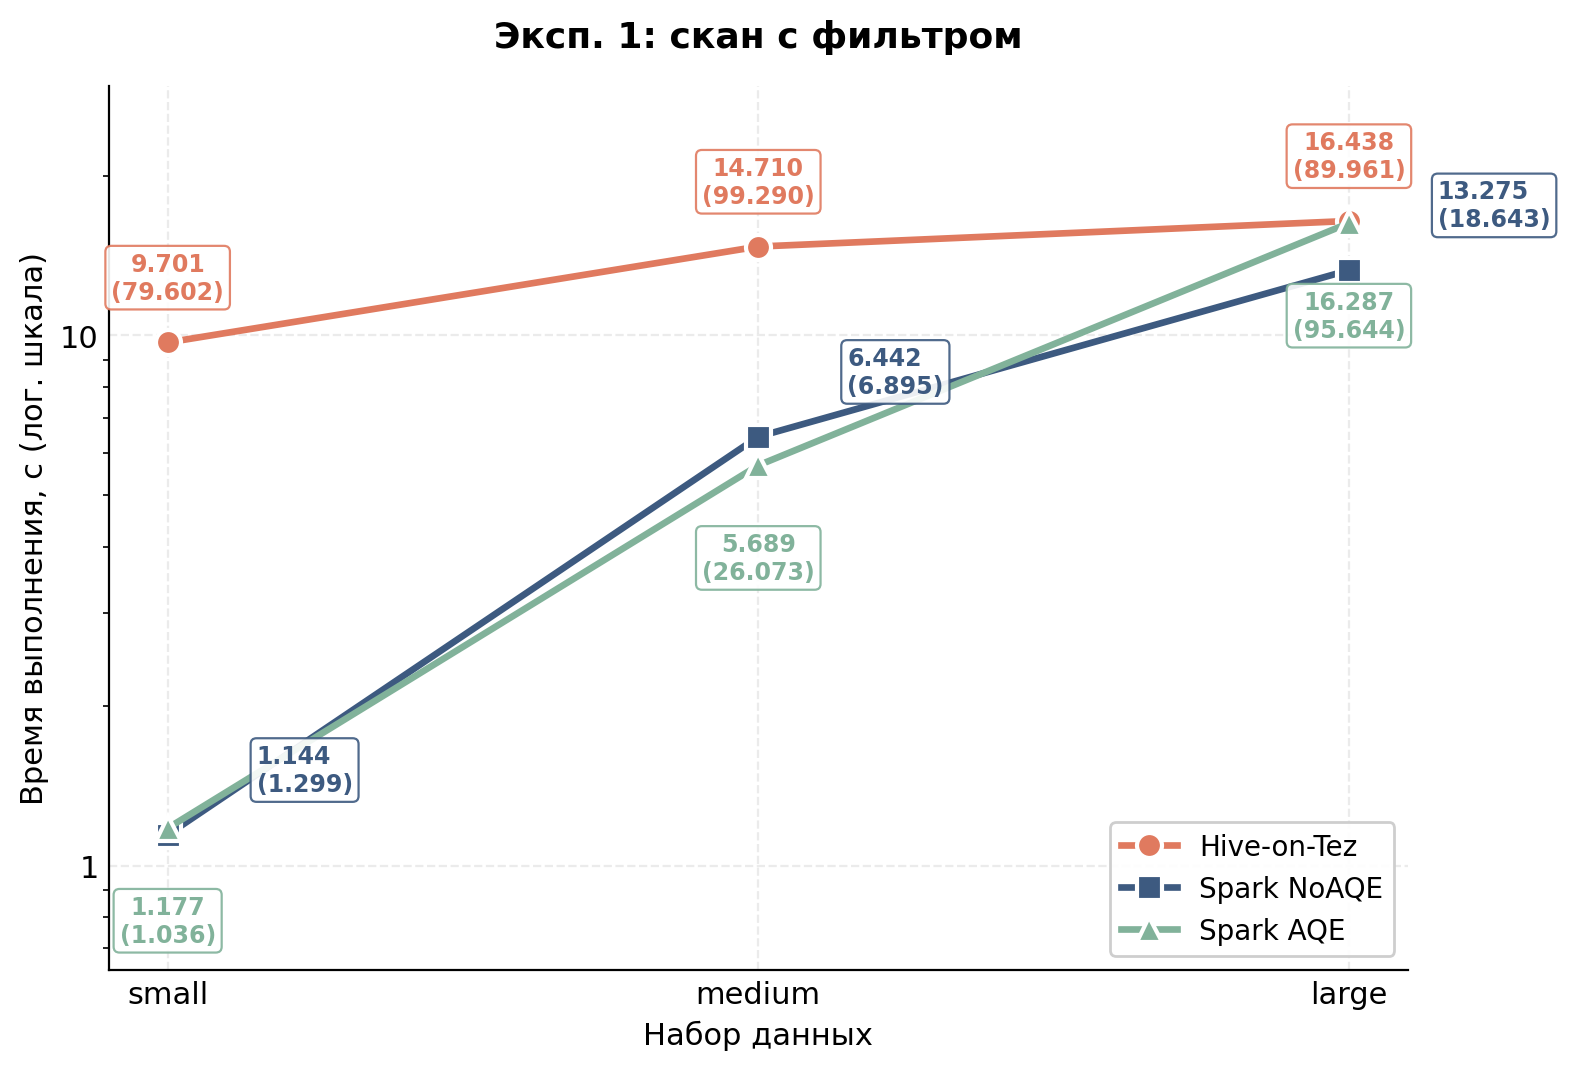
\includegraphics[width=0.85\textwidth]{graphs/exp1.png}
\caption{Эксперимент 1: время выполнения (медиана горячих прогонов; в скобках - холодный)}
\label{fig:q1}
\end{figure}

На нагрузке данного типа Spark существенно опережает Hive-on-Tez на малых и
средних объёмах: на наборе small разрыв достигает порядка величины (1.1 против
9.7~с). Причина - различие в накладных расходах на запуск: Hive-on-Tez
инициализирует контейнеры приложения через YARN, тогда как Spark переиспользует
уже поднятые исполнители. На лёгкой I/O-bound нагрузке именно эти накладные
расходы доминируют над собственно временем чтения. С ростом объёма (large)
разрыв сокращается, поскольку доля полезной работы растёт относительно
фиксированных издержек инициализации.

Конфигурации Spark с AQE и без него на данном запросе практически неразличимы
(на medium 5.7 против 6.4~с): запрос не содержит соединений и перекоса, поэтому
адаптивная оптимизация не находит применения. Это согласуется с природой
нагрузки - на чистом сканировании роль оптимизатора минимальна, а различия
определяются эффективностью чтения и издержками движка, а не стратегией
планирования.

Холодные прогоны заметно превышают горячие (для Hive - 79-99~с против 9-16~с),
что отражает первичную инициализацию исполнителей и компиляцию JIT при
непрогретом кэше. На разделяемом кластере состояние кэша не контролируется,
поэтому холодный прогон приводится справочно.

\subsection{Эксперимент 2: соединение с малой таблицей (broadcast join)}

\subsubsection{Запрос и назначение}
Второй запрос подсчитывает число субподрядчиков на контракт - левое соединение
основной таблицы с малой таблицей субподрядчиков (35\,тыс. записей) и
последующая группировка. Поскольку правая таблица мала, запрос проверяет, способен
ли стоимостный оптимизатор распознать малую сторону и выбрать broadcast-соединение
(рассылку малой таблицы на все узлы) вместо перемешивания основной таблицы.

\begin{lstlisting}[style=sparkconf, caption={Эксперимент 2}, label={lst:q2}]
SELECT c.contract_reg_num, COUNT(s.subcontractor_inn) AS subcontractor_count
FROM t_team_amkld.contracts_docs_<tier> c
LEFT JOIN t_team_amkld.subcontractors s
  ON c.contract_reg_num = s.contract_reg_num
GROUP BY c.contract_reg_num
\end{lstlisting}

\subsubsection{Анализ}
\begin{figure}[H]
\centering
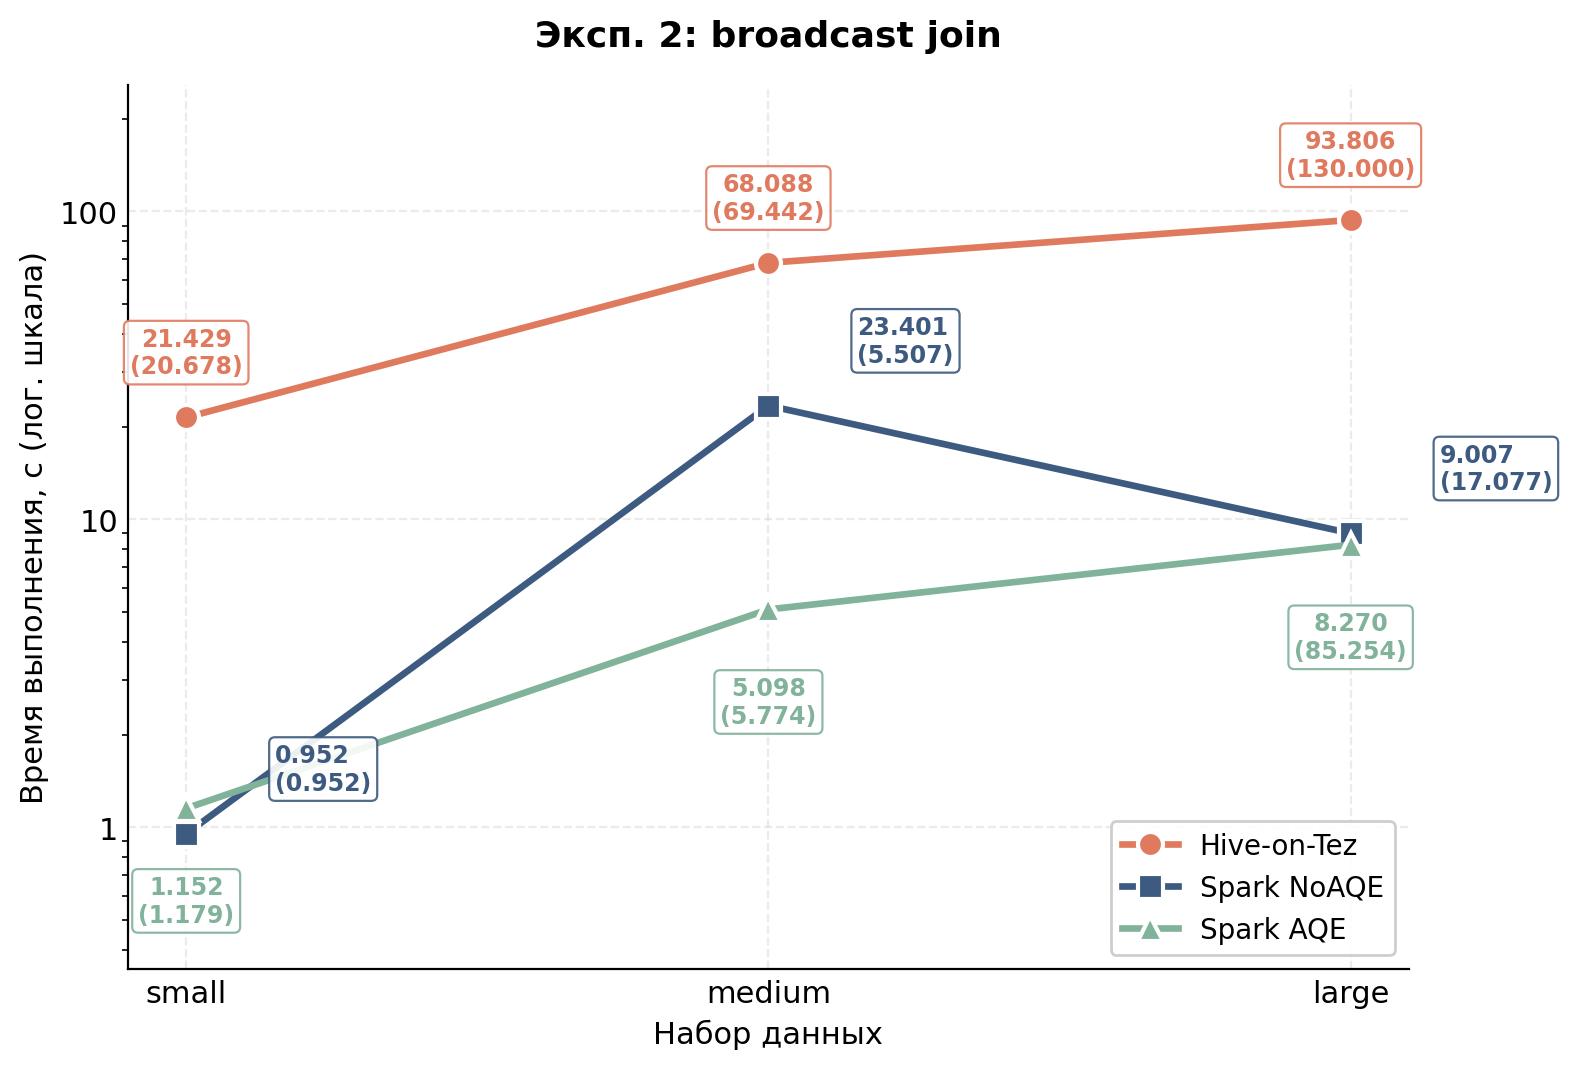
\includegraphics[width=0.85\textwidth]{graphs/exp2.png}
\caption{Эксперимент 2: время выполнения (медиана горячих прогонов; в скобках - холодный)}
\label{fig:q2}
\end{figure}

Малый размер таблицы субподрядчиков позволяет оптимизатору выбрать
broadcast-соединение, при котором перемешивание основной таблицы отсутствует.
В результате нагрузка остаётся лёгкой, и Spark вновь значительно опережает
Hive-on-Tez - на large 8-9 против 99~с (более чем в десять раз). Несмотря на
наличие в запросе соединения и группировки, перекос распределения по ключу
\texttt{contract\_reg\_num} здесь почти не проявляется: рассылка малой стороны
обходит перемешивание основной таблицы.

Конфигурации Spark с AQE и без него остаются близкими (на large 8.3 против
9.3~с): поскольку соединение выполняется через broadcast, адаптивная обработка
перемешивания не востребована. Единичные выбросы в горячих прогонах (например,
64.7~с среди прогонов Spark NoAQE на medium) обусловлены конкуренцией за ресурсы
разделяемого кластера и нивелируются медианой.

\subsection{Эксперимент 3: соединение с большой таблицей (shuffle join)}

\subsubsection{Запрос и назначение}
Третий запрос соединяет основную таблицу с таблицей этапов исполнения
(44\,млн записей) и подсчитывает число уникальных этапов на контракт с
сортировкой результата. В отличие от предыдущего, правая таблица слишком велика для broadcast-рассылки (её размер многократно превышает порог autoBroadcastJoinThreshold), поэтому соединение выполняется через shuffle join по ключу \texttt{contract\_reg\_num}. Запрос совмещает три
тяжёлые операции: перемешивание при соединении, дедупликацию
(\texttt{COUNT(DISTINCT)}) и глобальную сортировку. Это основной кейс для
проверки адаптивной оптимизации, поскольку перемешивание по ключу с перекосом
распределения - именно та ситуация, в которой AQE способен переоптимизировать
план в рантайме.

\begin{lstlisting}[style=sparkconf, caption={Эксперимент 3}, label={lst:q3}]
SELECT c.contract_reg_num, COUNT(DISTINCT s.agg_key_id) AS stages_count
FROM t_team_amkld.contracts_docs_<tier> c
LEFT JOIN t_team_amkld.stages s
  ON c.contract_reg_num = s.contract_reg_num
GROUP BY c.contract_reg_num
ORDER BY stages_count DESC
\end{lstlisting}

\subsubsection{Анализ}
\begin{figure}[H]
\centering
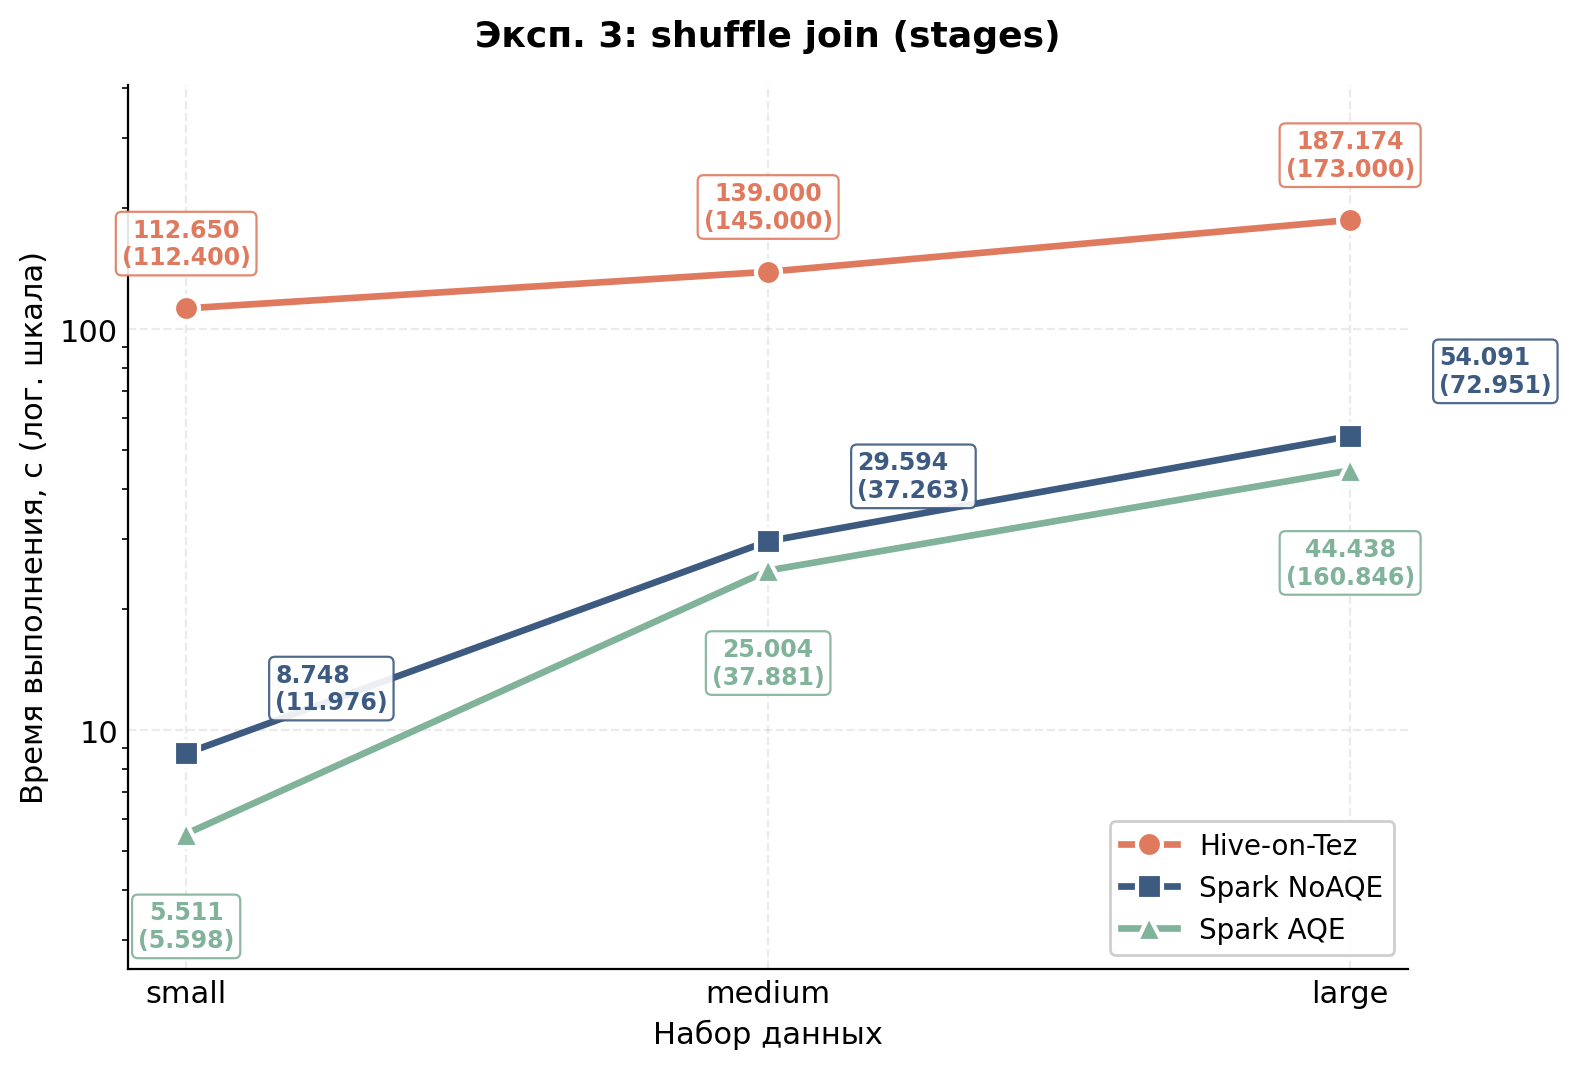
\includegraphics[width=0.85\textwidth]{graphs/exp3.png}
\caption{Эксперимент 3: время выполнения (медиана горячих прогонов; в скобках - холодный)}
\label{fig:q3}
\end{figure}

На тяжёлой нагрузке с перемешиванием картина меняется. Во-первых,
преимущество Spark над Hive-on-Tez сокращается: если на лёгких сканах разрыв
достигал порядка величины, то здесь на large Spark быстрее лишь в 3-4 раза
(44 против 185~с). Это объясняется тем, что при интенсивном перемешивании
архитектура Hive-on-Tez, активно использующая диск, меньше проигрывает, чем на
операциях, где доминируют накладные расходы на запуск.

Во-вторых, именно здесь проявляется эффект адаптивной оптимизации. На наборе
large конфигурация с AQE опережает конфигурацию без него (44.4 против 54.1~с,
выигрыш около 18\%): достаточный объём перемешиваемых данных позволяет AQE
окупить накладные расходы на рантайм-переоптимизацию. На меньшем наборе medium
эффект уже не столь однозначен, что указывает на наличие порога объёма, за
которым адаптивная оптимизация начинает себя оправдывать. Это согласуется с
результатами эксперимента~2, где при broadcast-соединении AQE не давал
выигрыша вовсе.

В-третьих, обращает на себя внимание стабильность Hive-on-Tez: разброс его
горячих прогонов минимален (на large 173-191~с), тогда как у Spark отдельные
прогоны заметно отклоняются. Hive-on-Tez демонстрирует предсказуемое, хотя и
более медленное, поведение, что может быть существенно для прогнозируемости
нагрузки.

\subsection{Эксперимент 4: извлечение даты регулярным выражением}

\subsubsection{Запрос и назначение}
Четвёртый запрос извлекает дату из текстового поля этапа исполнения с помощью
регулярного выражения - типичная для инженерии данных задача разбора
слабоструктурированных текстовых полей. Алгоритмически это нагрузка типа
CPU-bound: основная стоимость приходится на построчное применение регулярного
выражения, а не на ввод-вывод или перемешивание. Соединения и агрегации
отсутствуют. Запрос проверяет эффективность исполнения тяжёлых строковых
выражений - в частности, генерации кода (codegen) в Spark по сравнению с
исполнением выражений в Hive-on-Tez.

\begin{lstlisting}[style=sparkconf, caption={Эксперимент 4}, label={lst:q4}]
SELECT contract_reg_num,
       regexp_extract(docs_done_stage,
                      '(\\d{4}-\\d{2}-\\d{2})', 1) AS extracted_date
FROM t_team_amkld.contracts_docs_<tier>
WHERE docs_done_stage IS NOT NULL
\end{lstlisting}

\subsubsection{Анализ}
\begin{figure}[H]
\centering
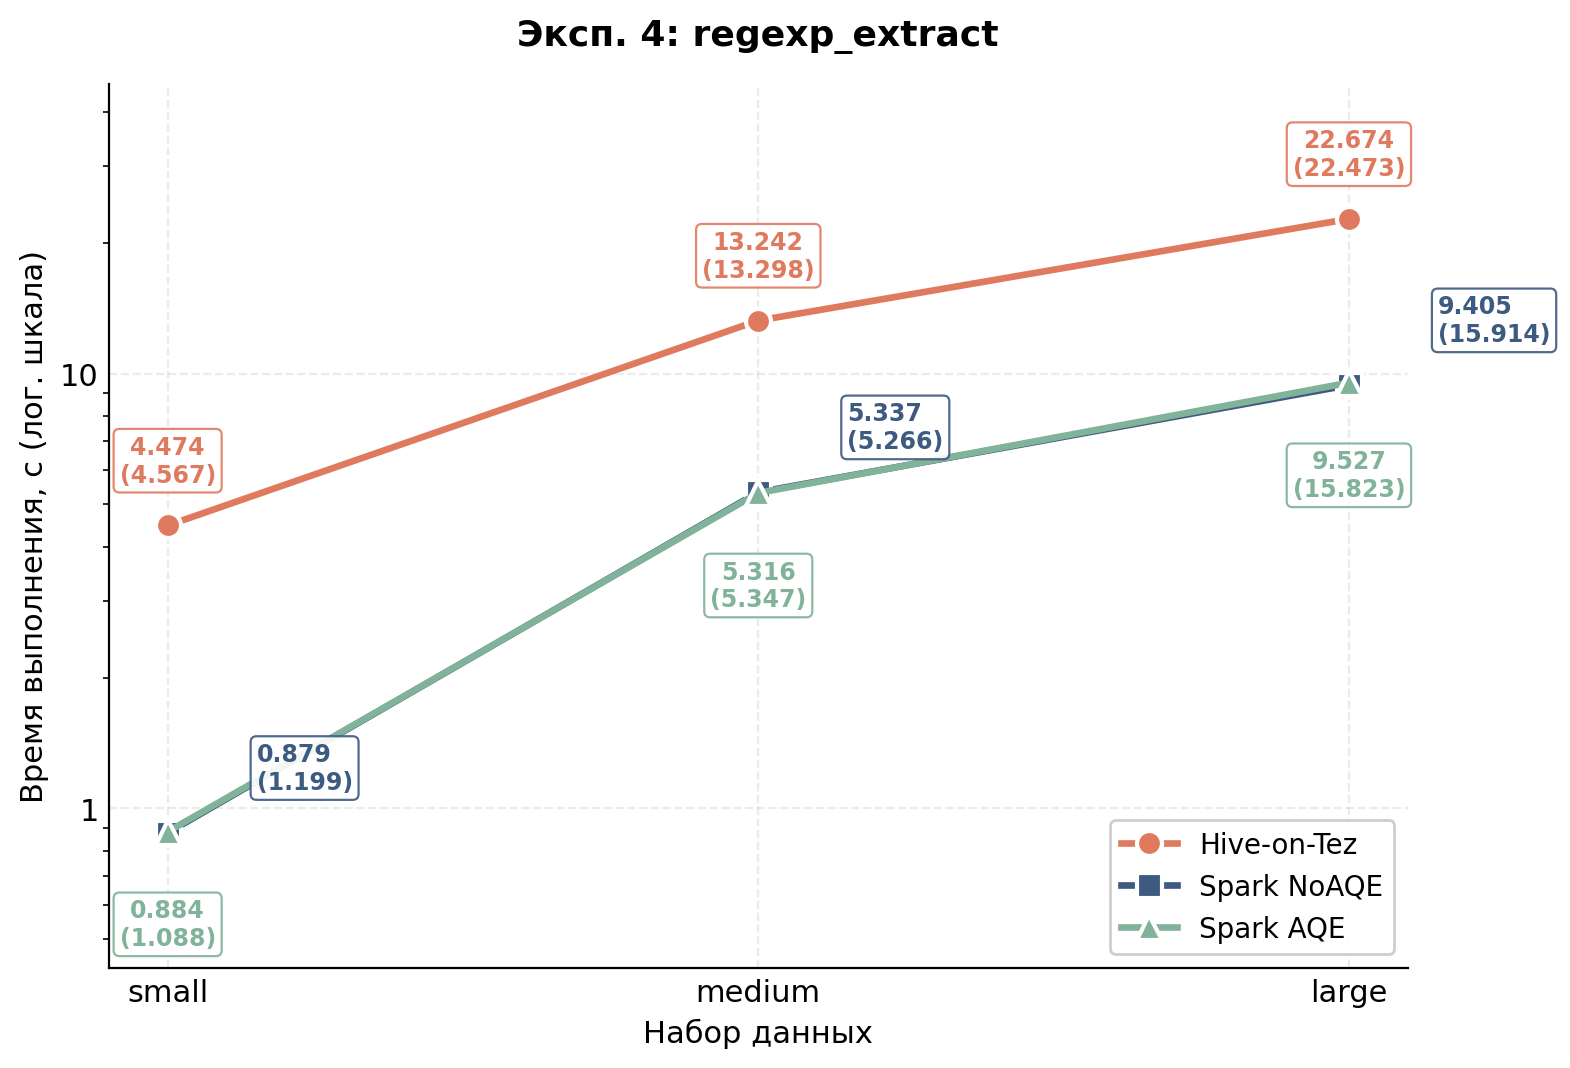
\includegraphics[width=0.85\textwidth]{graphs/exp4.png}
\caption{Эксперимент 4: время выполнения (медиана горячих прогонов; в скобках - холодный)}
\label{fig:q4}
\end{figure}

На CPU-bound нагрузке Spark стабильно опережает Hive-on-Tez, однако разрыв
умеренный - на large порядка 2.4 раза (9.4 против 22.5~с), что меньше, чем на
лёгких сканах. Преимущество объясняется генерацией кода в Spark: Catalyst
компилирует выражения в байт-код, что эффективнее на массовой построчной
обработке.

Конфигурации Spark с AQE и без него практически идентичны (на large 9.4 против
9.5~с) - результат, закономерный для нагрузки без соединений и перемешивания:
адаптивная оптимизация работает на границах перемешивания, которых здесь нет,
и потому не оказывает влияния. Это перекликается с экспериментом~1: на
нагрузках без перемешивания (как I/O-bound, так и CPU-bound) роль адаптивного
оптимизатора отсутствует, а различия определяются исключительно эффективностью
самих движков.

Характерно также, что у Hive-on-Tez холодный и горячий прогоны практически
совпадают (22.5 против 22.5~с), тогда как у Spark холодный прогон заметно выше
горячего (15.9 против 9.4~с). Это отражает разогрев JVM и компиляцию кода в
Spark при первом обращении, отсутствующие в Hive-on-Tez в той же мере.

\subsection{Эксперимент 5: приведение типов (string $\to$ date)}

\subsubsection{Запрос и назначение}
Пятый запрос приводит набор текстовых полей с датами к типу date - операция
нормализации, характерная для подготовки сырого слоя данных. Нагрузка
CPU-bound, но в отличие от предыдущего эксперимента она распределена по
нескольким столбцам и выполняется без фильтра, то есть обрабатывается весь
набор по полной проекции. Выполнение инициируется записью в формат-приёмник
noop, что вынуждает обработать все столбцы без материализации результата
(в отличие от подсчёта строк, при котором лишние столбцы могли бы быть
отсечены).

\begin{lstlisting}[style=sparkconf, caption={Эксперимент 5}, label={lst:q5}]
SELECT contract_reg_num,
       TO_DATE(dt_contract,       'yyyy-MM-dd') AS dt_contract_d,
       TO_DATE(start_dt_contract, 'yyyy-MM-dd') AS start_d,
       TO_DATE(end_dt_contract,   'yyyy-MM-dd') AS end_d,
       TO_DATE(dt_signing,        'yyyy-MM-dd') AS signing_d,
       TO_DATE(termination_dt,    'yyyy-MM-dd') AS termination_d
FROM t_team_amkld.contracts_docs_<tier>
\end{lstlisting}

\subsubsection{Анализ}
\begin{figure}[H]
\centering
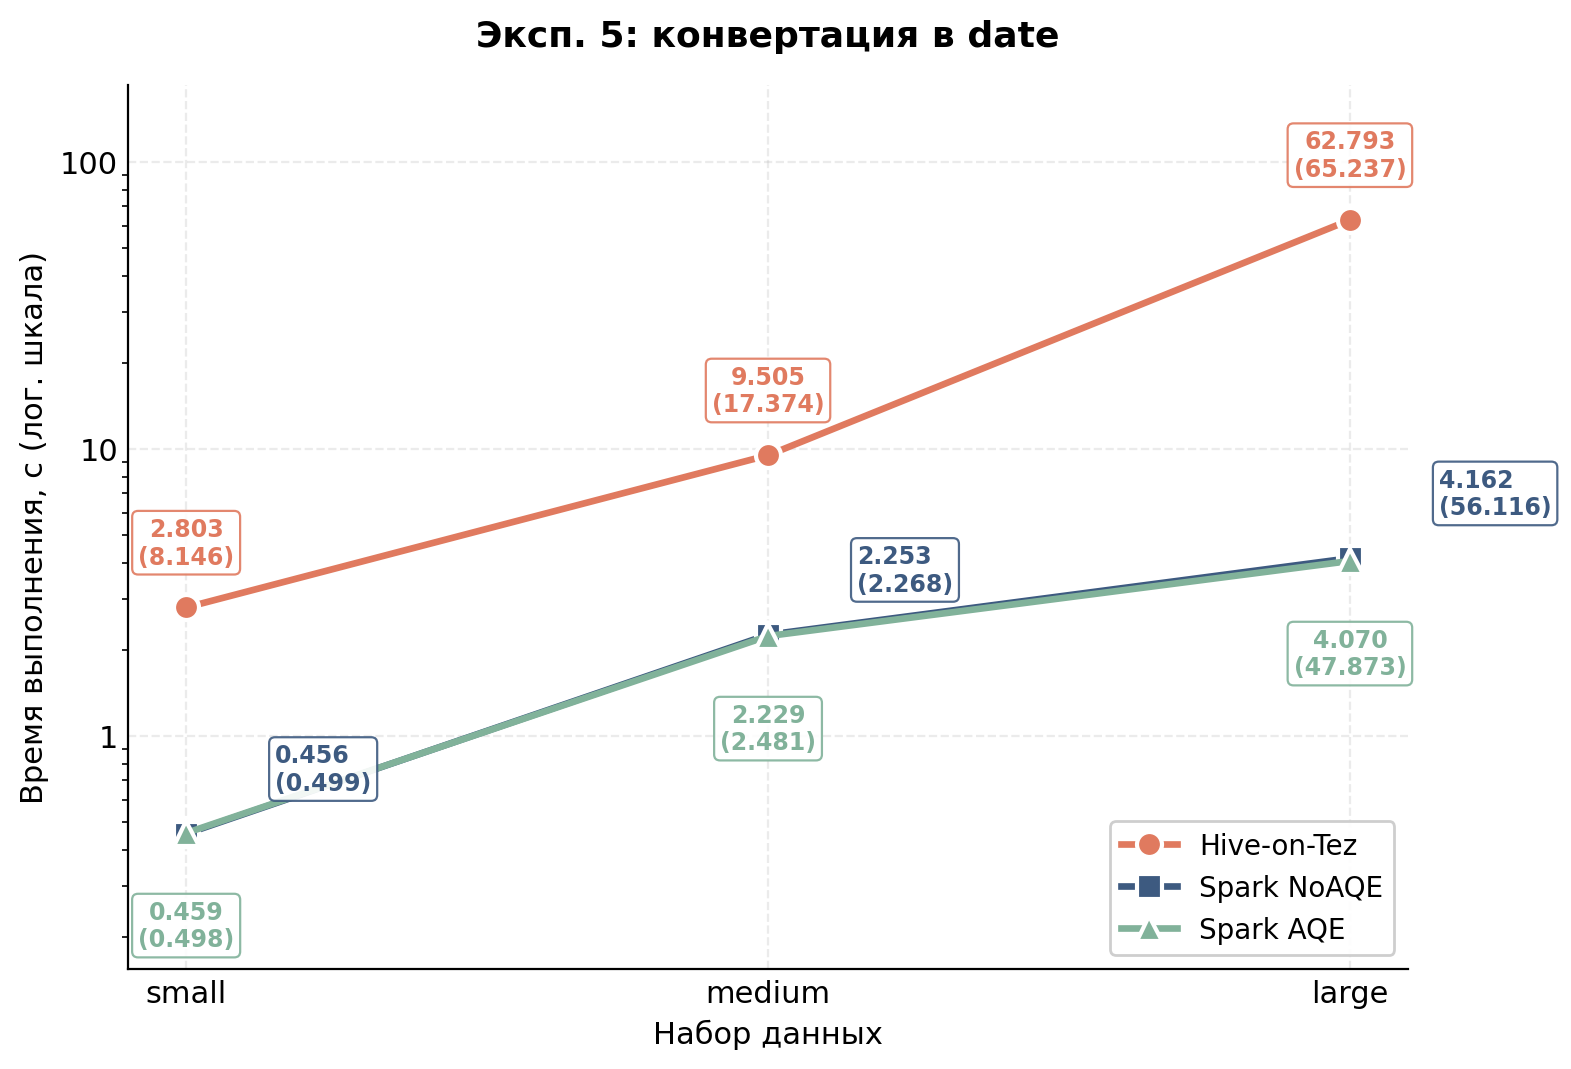
\includegraphics[width=0.85\textwidth]{graphs/exp5.png}
\caption{Эксперимент 5: время выполнения (медиана горячих прогонов; в скобках - холодный)}
\label{fig:q5}
\end{figure}

Приведение типов по широкой проекции даёт наибольший разрыв между движками: на
large Spark выполняет запрос примерно за 4~с против 65~с у Hive-on-Tez - более
чем в пятнадцать раз быстрее. Столь значительное преимущество объясняется
эффективностью генерации кода Spark при массовом приведении типов по множеству
столбцов: Catalyst компилирует преобразования в байт-код, тогда как
Hive-on-Tez обрабатывает выражения существенно медленнее.

Конфигурации Spark с AQE и без него вновь неразличимы (на large 4.1 против
4.2~с), что ожидаемо для нагрузки без перемешивания и подтверждает общую
закономерность: адаптивная оптимизация значима лишь при наличии операций
перемешивания.

Холодные прогоны Spark на large заметно превышают горячие (56 против 4~с) -
проявление разогрева JVM, тогда как у Hive-on-Tez холодный и горячий прогоны
сопоставимы. Эта закономерность устойчиво наблюдается во всех экспериментах:
Spark достигает высокой производительности лишь после разогрева, тогда как
Hive-on-Tez демонстрирует стабильное во времени, но более медленное поведение.

\section{Заключение}

Мы провели сравнение производительности и ресурсоёмкости двух движков
пакетной обработки больших данных, Hive-on-Tez и Apache Spark, на реальных
данных государственных контрактов (zakupki.gov.ru). Сравнение выполнено на трёх
наборах данных нарастающего объёма и пяти запросах, покрывающих различные типы
вычислительной нагрузки (I/O-bound, CPU-bound, операции с перемешиванием), при
выравненном ресурсном бюджете и с раздельным анализом конфигураций Spark с
адаптивной оптимизацией (AQE) и без неё.

Для наглядности сведём итоги всех проведённых экспериментов в единую таблицу.
В табл.~\ref{tab:summary} приведены финальные результаты измерений по всем пяти
запросам, трём конфигурациям и трём наборам данных: основным значением служит
медиана горячих прогонов, в скобках указан холодный прогон.

\begin{table}[ht]
\centering
\caption{Сводные результаты: медиана горячих прогонов, с (в скобках - холодный)}
\label{tab:summary}
\scriptsize
\setlength{\tabcolsep}{3pt}
\begin{tabular}{|l|r|r|r|r|r|r|r|r|r|}
\hline
& \multicolumn{3}{c|}{\textbf{Hive-on-Tez}}
& \multicolumn{3}{c|}{\textbf{Spark NoAQE}}
& \multicolumn{3}{c|}{\textbf{Spark AQE}} \\
\cline{2-10}
\textbf{Эксперимент} & S & M & L & S & M & L & S & M & L \\
\hline
1. Скан с фильтром & 9.7\,(79.6) & 14.7\,(99.3) & 16.4\,(90.0) & 1.1\,(1.3) & 6.4\,(6.9) & 13.3\,(18.6) & 1.1\,(1.0) & 5.7\,(26.1) & 16.3\,(95.6) \\
2. Broadcast join & 21.4\,(20.7) & 68.1\,(69.4) & 98.7\,(130) & 1.0\,(1.0) & 5.4\,(5.5) & 9.3\,(17.1) & 1.2\,(1.2) & 5.1\,(5.8) & 8.3\,(85.3) \\
3. Shuffle join & 112.6\,(112) & 139\,(145) & 187.2\,(173) & 9.1\,(12.0) & 29.6\,(37.3) & 54.1\,(73.0) & 5.5\,(5.6) & 25.0\,(37.9) & 44.4\,(161) \\
4. regexp\_extract & 4.5\,(4.6) & 13.2\,(13.3) & 22.5\,(22.5) & 0.9\,(1.2) & 5.3\,(5.3) & 9.4\,(15.9) & 0.9\,(1.1) & 5.3\,(5.3) & 9.5\,(15.8) \\
5. Конвертация date & 2.8\,(8.1) & 9.5\,(17.4) & 62.8\,(65.2) & 0.5\,(0.5) & 2.2\,(2.3) & 4.2\,(56.1) & 0.5\,(0.5) & 2.2\,(2.5) & 4.1\,(47.9) \\
\hline
\end{tabular}
\end{table}

В целом полученные результаты подтверждают вывод предыдущей работы о том, что
Spark превосходит Hive-on-Tez по производительности: на всех пяти типах нагрузки
и всех объёмах данных Spark показал меньшее время выполнения. Вместе с тем
величина этого преимущества существенно зависит от характера запроса. На лёгких
сканах и операциях без перемешивания разрыв достигает порядка величины, что
объясняется как меньшими накладными расходами на запуск (переиспользование
исполнителей против инициализации контейнеров через YARN), так и эффективной
генерацией кода в Spark на построчной обработке. На тяжёлых операциях с
перемешиванием преимущество сокращается до 3-4 раз, поскольку при интенсивном
обмене данными архитектура Hive-on-Tez, активно использующая диск, проигрывает
меньше.

Эффект адаптивной оптимизации (AQE) проявляется избирательно. На нагрузках без
перемешивания (сканы, построчные преобразования) AQE не оказывает влияния, так
как переоптимизация плана выполняется на границах перемешивания, которые в
таких запросах отсутствуют. На соединении большой таблицы с перемешиванием AQE
даёт ощутимый выигрыш на наибольшем наборе данных, тогда как на меньших объёмах
накладные расходы адаптации не окупаются. Это указывает на наличие порога
объёма, за которым адаптивная оптимизация начинает себя оправдывать.

Отдельно отмечены два свойства, важных для практики. Во-первых, Hive-on-Tez
демонстрирует значительно более стабильное время выполнения от прогона к
прогону, тогда как Spark при более высокой средней производительности
показывает большую вариативность, что может быть существенно для задач с
требованиями к предсказуемости. Во-вторых, во всех экспериментах прослеживается
чёткая тенденция: холодный прогон превышает горячие. У Spark этот разрыв
особенно выражен (на отдельных запросах холодный прогон в десятки раз медленнее
горячего, например 56 против 4~с на эксперименте~5), что обусловлено разогревом
JVM и компиляцией кода при первом обращении. У Hive-on-Tez та же тенденция
присутствует, хотя выражена слабее: на части запросов холодный и горячий прогоны
сопоставимы, на других (например, скан с фильтром) холодный прогон также заметно
выше. Это означает, что для обоих движков первое обращение к данным обходится
дороже установившегося режима, и при оценке производительности холодный старт
следует учитывать отдельно.

\subsection{Рекомендации по применению}

На основе полученных результатов можно сформулировать практические рекомендации
по выбору движка.

Если заранее известно, что объём обрабатываемых данных невелик, использование
Hive-on-Tez вполне оправдано: на малых наборах оба движка справляются быстро,
разница в абсолютном времени несущественна для большинства задач, а Hive-on-Tez
дополнительно обеспечивает более предсказуемое время выполнения и не требует
переиспользования сессии для достижения стабильной производительности.

В общем случае, особенно при средних и больших объёмах данных, предпочтительным
является Spark: он стабильно опережает Hive-on-Tez на всех типах нагрузки, а на
операциях без перемешивания (сканирование, построчные преобразования,
приведение типов) преимущество достигает порядка величины.

Если известно, что нагрузка содержит соединения больших таблиц с перемешиванием
по ключу, подверженному перекосу распределения (skew), рекомендуется включать
адаптивную оптимизацию (AQE): эксперименты подтвердили, что на достаточно
больших объёмах она улучшает производительность соединений с перемешиванием. На
нагрузках без перемешивания включение AQE безвредно, но и не даёт выигрыша,
поэтому его можно оставлять активным по умолчанию.

В качестве направлений дальнейшей работы можно выделить расширение набора
запросов до полноценного бенчмарка (например, TPC-DS) для сопоставимости с
другими исследованиями, измерение поведения при конкурентном исполнении
нескольких запросов, а также прицельное изучение обработки перекоса
распределения средствами адаптивной оптимизации.

\end{document}


